\documentclass[a4paper,11pt]{article}
\usepackage{amsmath}
\usepackage{wrapfig}
\usepackage{fancyhdr}
\usepackage{graphicx}
\usepackage{url}
\usepackage{float}
\usepackage{amsmath}
\usepackage{amssymb}
\usepackage[margin=1in]{geometry}

%\setlength{\voffset}{-0.5in}
%\setlength{\headsep}{5pt}
\newcommand{\suchthat}{\;\ifnum\currentgrouptype=16 \middle\fi|\;}


%===========---------================
% Author John H Allard
% CMPE 12, Lab #1 Write-up
% October 9th, 2014
%===========---------================


\title{ CMPE 12 Lab Report \# 1 \\[7 in]}
\author{John Allard \\ TUTOR \\ Lab Section \#2}
\date{October 6th, 2014}

\begin{document}
\maketitle
\newpage
\tableofcontents
\newpage

%*************************************%
%************* OVERVIEW **************%
%*************************************%

\section{Overview}
This lab served as an introduction to circuit design from truth tables using logic gates. All circuits were implemented using the free MultiMedia Logic (MML) program, which allows the user to drag, drop, and connect different circuit components. After the circuit is connected it can be simulated to help check for design errors. This lab consisted of 4 section, with each section varying in difficulty and length. 



%*************************************%
%************** PART A ***************%
%*************************************%

\section{Part A : Using MultiMedia Logic}
\subsection{Procedure}
This section was a combined introduction to MML and DeMorgan's laws. To start we were instructed to navigate to an MML tutorial on YouTube\footnote{\url{http://www.youtube.com/watch?v=hJq2gECXYWc&noredirect=1}} and build the circuit that is shown in the tutorial. After this, we were instructed to show our understanding of MML by implementing DeMorgans laws \(A'B' = (A+B)'\). To do this, we needed to build a circuit for each side of the DeMorgans equation and show their equivilence both in practice and by truth table. 
\subsection{Results}
\subsubsection{Results - Tutorial} 
 \begin{wrapfigure}{r}{0.68\textwidth}
     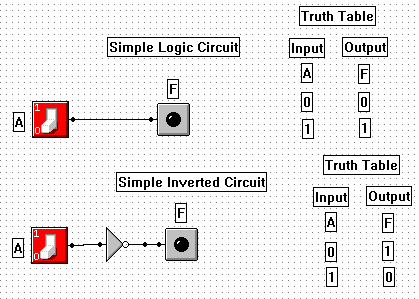
\includegraphics[width=4.4in]{PartACircuit}
   \caption{Circuits for Part A Tutorial.}
   \label{fig:tutorial}
\end{wrapfigure} 
To start, we completed an extremely simple circuit using the MML software. This circuit is about as simple as one can get, it is just a binary switch connected to an LED. In this case, if the switch is high, the LED is on, if the switch is low, the LED is off. Next we simply inserted an NOT between the switch and the LED, causing it to only light up when the switch is in a low state. The two circuits for the tutorial section of part A can be seen in figure one. 

\subsubsection{Results - DeMorgans Law} 
Our next goal was to create two new circuits which demonstrate DeMorgans law, specifically the fact that \(A'B' = (A+B)'\). This involved the use of two switches, labled $A$ and $B$. These switches will be used as the inputs for two circuits, the first one representing $A'B'$ and the second one representing $(A+B)'$.
\begin{figure}[h!]
   \centering
     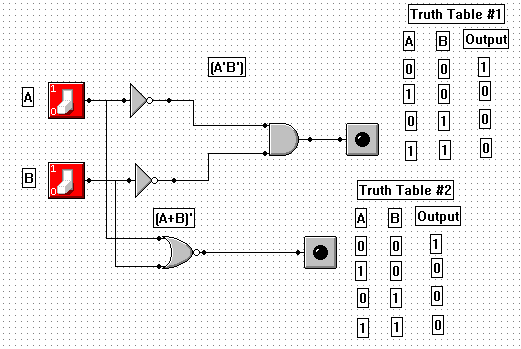
\includegraphics[width=5in]{PartADM}
   \caption{Circuits for Part A2, Showing DeMorgans Law.}
   \label{fig:parta2}
\end{figure}  
Once completed, a simulation of these circuits can be run and it can be seen that the LED for each of the two circuits are in an identical state for the entirety of the message space, which happens to only be $ \lbrace 00, 01, 10, 11 \rbrace $ for this simple example. The first circuit, $A'B'$, is created by passing the $A$ and $B$ inputs through NOTs before combining them into an AND gate. The output of the AND gate is run directly to an LED. The second circuit is made by running the $A$ and $B$ inputs directly into a NOR gate, then to an LED. The circuit and truth tables can be seen in Figure \ref{fig:parta2}. \\




%*************************************%
%************ PART B *****************%
%*************************************%

\section{Part B : Implementing Functions as Sums of Products}
\subsection{Procedure}

\begin{wrapfigure}{l}{0.37\textwidth}
   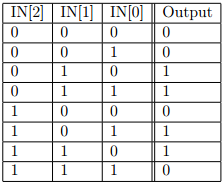
\includegraphics[width=2in]{PartBTT}
   \caption{Truth Table for Parts B and C}
   \label{fig:partbtt}
\end{wrapfigure} 

This part of the lab consisted of two sections, B1 and B2. The goal of both sections was the same, implement the truth table in Figure \ref{fig:partbtt}, the differences between the two implementations are the restrictions on the gates that can be used. \par
In the circuits that we are building, the following names will be used for the inputs listed in Figure \ref{fig:partbtt} : 
\[ \text{IN[2] $\to A$, IN[1] $\to B$, IN[0] $\to C$} \] 
The output of the circuit will be a single LED with a basic $1 = \text{HIGH}$, $0 = \text{LOW}$ relationship. Part B1 asked us to construct a circuit to represent the truth table in Figure \ref{fig:partbtt} using AND, OR, or NOT gates. Part B2 asked us to reimplement the same circuit using only NAND gates. This requires translation of the AND, OR, and Inversion gates into nested layers of NAND gates. Finally, we were supposed to run the circuits in both sections side by side to ensure their equivalence. 

\subsection{Results}
Before any circuitry could be properly constructed, the truth table had to be broken down into a boolean equation using the sum of products rule. Working from left to right in the truth table in Figure \ref{fig:partbtt}, with $\text{IN[2]} \to A$, $\text{IN[1]} \to B$, $\text{IN[0]} \to C$, we arrive at the following equation.
 \begin{equation}\label{eq:one} \text{A'BC'} + \text{A'BC} + \text{AB'C} + \text{ABC'} \end{equation}

\subsubsection{Results - AND, OR, \& NOT Gates} 
Part B1 involved directly translating \eqref{eq:one} into a circuit using MML. Because we were allowed to use AND, OR, and NOT gates, the circuit reads all most exactly like \eqref{eq:one}. The circuit for part B1 is shown in figure 4.

\begin{figure}[h!]
   \centering
     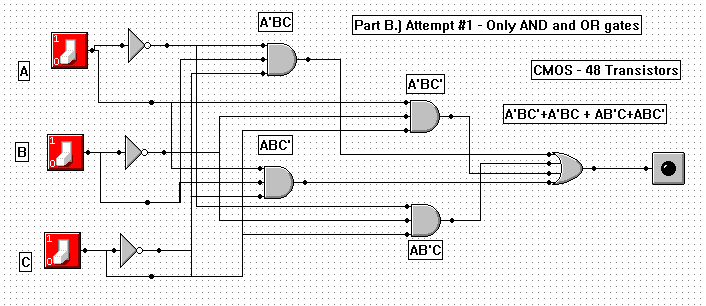
\includegraphics[width=6in]{PartB1Circuit}
   \caption{Circuit for Part B1}
   \label{fig:b1circuit}
\end{figure} 

The circuit is best read from left to right. It starts off with the three inputs, $A$, $B$, and $C$. These three switches can be toggled to create a total of $2^3 = 8$ possible combinations. Right of these switches is a layer of four 3-input AND gates. These AND gates represent the individual products in \eqref{eq:one}. The output from each of these four AND gates are routed to a single 4-input OR gate. This gate represents the sum of the individual products shown in \eqref{eq:one}. The output of this OR gate is connected to a single LED to display the circuit output to the user. As is shown in figure 4, this circuit consists of a total of 48 transistors using CMOS transistor logic. How I found this number is documented below.
\[ \text{\# of* Transistors per Gate}\]
\[ \text{NOT} = 2 \text{, AND} = 2n_1+2 \text{, OR} = 2n_2+2 \]
Where $n$ denotes the number of inputs for that specific gate. With 3 NOT gates, four 3-input AND gates, and one 4-input OR gate, the linear combination of transistors for this circuit becomes \ldots
\[ 3*(\text{NOT})+4*(\text{AND})+1*(\text{OR}) = \]
\[ 3*2+4*(2*n_1+2)+1*(2*n_2+2) = 6+32+10 = 48\]
Of course in the real world we would not use 48 transistors for this circuit, \eqref{eq:one} can be simplified significantly, as we will see in Part C.
\par

\subsubsection{Results - NAND Gates}
Next we were instructed to take \eqref{eq:one}, implement it in a circuit using MML, but this time we were only permitted to use NAND gates. I started with the circuit in the previous section (Figure 4), and used the following substitutions to achieve the same output with only NAND gates.
\[ \text{NOT($A$) $\to$ NAND($A$,$A$) }\]
\[ \text{AND($A$,$B$) $\to$ NAND($x$, $x$), where $x = $NAND($A$,$B$) } \]
\[ \text{OR($A$,$B$) $\to$ NAND($x_A$, $x_B$) where $x_n = $NAND($n$,$n$) }\]
We simulate an inverter by routing a single signal to both inputs of a NAND gate. If the signal is high, both inputs to the NAND are high, which outputs a 0. If the signal is low, both inputs are low and thus the NAND outputs a 1.
I simulate an AND gate by first routing two inputs through a single NAND gate. I then route this output to both inputs of another NAND gate. This effectively creates a `double negative` effect, canceling out the `N` in NAND.
Finally, I simulate an OR gate by routing each of the inputs through a NOT gate (which is just a NAND gate with one signal tied to both inputs), then finally routing the output from each NOT gate through a single NAND gate. This works because NAND only returns true if any input is 0. Because we inverted every input before the final NAND gate, this means that our NAND gate will only return true if any of the original signals were equal to 1, which is exactly the definition of an OR gate.

After I figured how to how to convert each individual component from the first circuit to their NAND gate equivalent, all that was left to do was to tie all of the NAND gates together and hope for the best. My final circuit is shown in Figure \ref{fig:b2circuit}.  

\begin{figure}[h!]
   \centering
     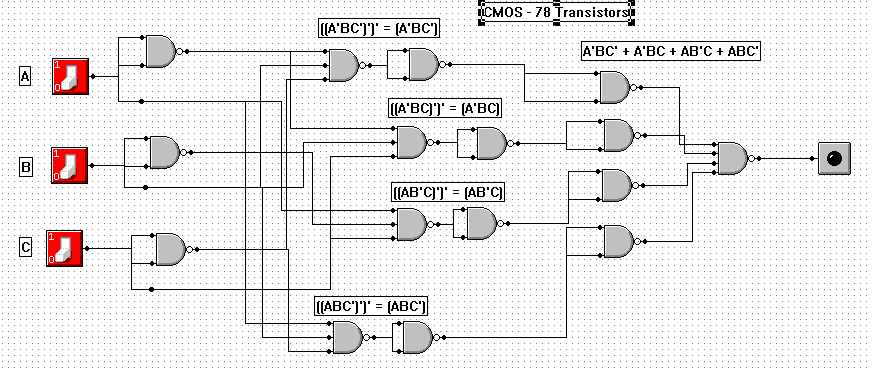
\includegraphics[width=6.5in]{PartB2}
   \caption{Circuit for Part B2, using only NAND gates.}
   \label{fig:b2circuit}
\end{figure}   
As you can see it consists only of NAND gates, yet structurely resembles the circuit from Figure \ref{fig:b1circuit}. It still has a layer of 3 NOT gates, followed by four 3-input AND gates, and lastly all 4 signals are tied together through an OR gate, the only difference was this time everything has been implemented using only NAND gates. The transistor count for this circuit was 78. I used the following math to find this number. 
\[ \text{\# of Transistors per Gate}\]
\[ \text{NAND} = 2n \]
Where $n$ denotes the number of inputs for the NAND gate. With eleven 2-input NAND gates, four 3-input NAND gates, and one 4-input NAND gate, the linear combination of transistors for this circuit is \ldots
\[ 11*(\text{NOT})+4*(\text{AND})+1*(\text{OR}) = \]
\[ 11*(2*2)+4*(2*3)+1*(2*4) = 44+24+10 = 78\]
\par

You can simulate these two circuits by running the \url{lab1B.lgi} file included with this paper.


%*************************************%
%************ PART C *****************%
%*************************************%

\section{Part C : Logic Minimization}
\subsection{Procedure}
The main goal of this section is to use the rules of Boolean algebra to simplify \eqref{eq:one} down to a more managable equation, then implement it again as a more simple circuit. For reference, here again is the equation we are simplifying.
\[ \text{A'BC'} + \text{A'BC} + \text{AB'C} + \text{ABC'} \]
\subsection{Results}
\subsubsection{Simplification}
I started by reducing down \eqref{eq:one} using Boolean algebra. My steps are listed below.
 \[ \text{A'BC'} + \text{A'BC} + \text{AB'C} + \text{ABC' \qquad  (original)} \]
 \[ \text{A'B(C' $+$ C) $+$ A(B'C $+$ BC') \qquad (factoring)} \]
 \[ \text{A'B(1) $+$ A(B'C $+$ BC')  \qquad (($X+X$') is a tautology)} \]
 \[ \text{A'B(1) $+$ $A$($B \oplus C$)  \qquad (($X$'$Y$+$XY$') $=$ XOR = $\oplus$)} \]
\begin{equation} \label{eq:two} \text{A'B $+$ $A$($B \oplus C$)} \end{equation}
The final simplified equation that I ended up with is \eqref{eq:two}. Beyond this point simplification is no longer possible, but the equation has still been reduced from its original form by quite a bit.

\subsubsection{Building the Circuit}
Now we were instructed to build a circuit corresponding to \eqref{eq:two}, which is equivilent to \eqref{eq:one}, which is derived from the truth table in Figure \ref{fig:partbtt}. So \eqref{eq:two} is just another way of representing the original truth table (Figure \ref{fig:partbtt}). This can be seen in Figure \ref{fig:partc}.
 \begin{figure}[h!]
   \centering
     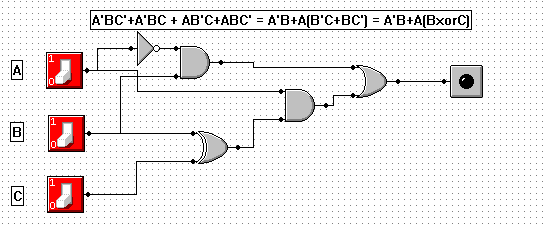
\includegraphics[width=6.5in]{partc}
   \caption{Part C, Simplified Circuit.}
   \label{fig:partc}
\end{figure}   
If you visually compare Figures \ref{fig:b2circuit} and \ref{fig:partc}, you can see how much simpler the latter is.This circuit performed identically when tested side by side with both circuits from Part B. 




%*************************************%
%************ PART D *****************%
%*************************************%

\section{Part D : Guessing Game}
\subsection{Procedure}
This section instructed us to design a 2-bit guessing game. The game works as follows  :
\begin{itemize}
\item User can set the value of two bits to either 0 or 1, giving them 4 combinations to make. 
\item Once the user's guess is set, they press a push button to start the game.
\item The button causes the a circuit component to generate a 2-bit random number.
\item This random number is compared to the users guess for equality.
\item If they are equal, an LED goes HIGH. If they are not, the LED stays low.
\end{itemize}

This involved comparing the low bits for equality, then comparing the high bits for equality, then finally checking that both of those comparisons returned true. If everything works right, the user should have a $\frac{1}{4}$ chance of winning.
\subsection{Results}
The trickiest problem in completing this part of the lab was figuring out how to compare two bits for equality. I know that AND returns true if they are both 1, which is partly correct. But AND returns 0 if they are both 0, which is not true. Then I realized that XOR is close to what we want, it only returns true if the two inputs are different, and returns false if they are the same. This is exactly the opposite of the desired functionality, so I simply decided to add a NOT gate at the end of an XOR gate to create an XNOR gate 
\[ \text{XNOR $=$ ($A \oplus B$)'}\]
So to start, we route the high bit from the user and the high bit from the random number to an XNOR gate, which returns 1 if they are equal and 0 otherwise. We then do the same thing with the low bits from the user's guess and random number. Finally, we route the output from both of these XNOR gates to a final AND gate, which will only output true if both inputs are true. The output from this AND gate is routed to a simple LED to let the user know if they have won or not.

\begin{figure}[h!]
   \centering
     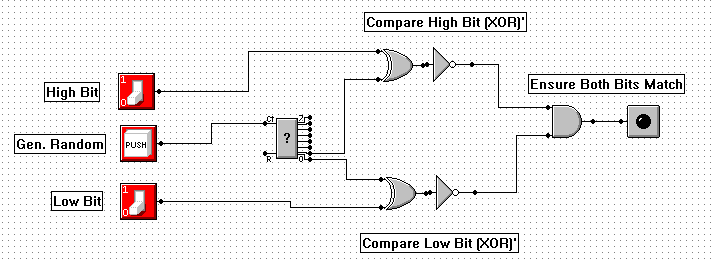
\includegraphics[width=6.5in]{partd}
   \caption{Part D Guessing Game Circuit}
   \label{fig:partd}
\end{figure}   

%*************************************%
%*********** CONCLUSION **************%
%*************************************%

\section{Conclusion}
This lab served as an introduction to building virtual circuits using the MultiMedia Logic program. In learning to use this program, we also learned to use truth tables to design circuits. After this we saw how the tools of Boolean algebra can allow us to significantly simplify the number of components in a given circuit by removing redundancies. Finally, we learned how to compare bits and use a random number generator in our circuit design. 

\end{document}